\documentclass[10pt, twocolumn]{article}

\usepackage[margin=0.75in]{geometry}
\usepackage{graphicx}
\usepackage{amsmath, amssymb}
\usepackage{booktabs}
\usepackage{caption}
\usepackage[hidelinks]{hyperref}
\usepackage{url}
\usepackage[numbers,sort&compress]{natbib}
\usepackage{listings}
\usepackage{xcolor}
\usepackage{titlesec}

\captionsetup{font=small, labelfont=bf, skip=4pt}
\titlespacing*{\section}{0pt}{6pt}{2pt}
\titlespacing*{\subsection}{0pt}{4pt}{1pt}
\setlength{\parskip}{2pt}
\setlength{\parindent}{0pt}
\setlength{\columnsep}{18pt}
\setlength{\textfloatsep}{6pt}
\setlength{\intextsep}{4pt}

\lstset{
  basicstyle=\ttfamily\footnotesize,
  keywordstyle=\color{blue!70!black},
  commentstyle=\color{gray},
  stringstyle=\color{orange!80!black},
  showstringspaces=false,
  breaklines=true,
  language=Python,
  xleftmargin=2pt,
  aboveskip=3pt, belowskip=3pt
}

\title{\vspace{-1.2cm}\textbf{\large On Adversarial Attacks and Defenses in Deep Learning:\\ A Systematic Study on MNIST}}
\author{\normalsize Wang Wenxuan \quad\textbar\quad Student ID: 1397228 \\
\small CDS521 Foundation of AI \quad\textbar\quad Deadline: 24 April 2026}
\date{\vspace{-1em}}

\begin{document}
\maketitle
\thispagestyle{empty}

\begin{abstract}
\small
Deep neural networks, despite super-human accuracy on vision benchmarks, can be fooled by imperceptibly small perturbations crafted by adversaries. This dissertation surveys the threat model, taxonomy, and defenses of \emph{adversarial machine learning}, and reports a controlled empirical study on MNIST. Using a four-layer convolutional classifier (421\,K parameters) trained on an NVIDIA RTX~2050 GPU, we (i)~implement the Fast Gradient Sign Method (FGSM) and Projected Gradient Descent (PGD) as white-box $L_\infty$ attacks, (ii)~compare them against a Madry-style PGD adversarially trained variant, and (iii)~analyze class-level vulnerability and compute cost. At $\varepsilon\!=\!0.3$, PGD-20 reduces the baseline's accuracy from $\mathbf{98.88\%}$ to $\mathbf{2.36\%}$, whereas the adversarially trained model retains $\mathbf{82.95\%}$. Adversarial training costs $\approx\!6$\,pp in clean accuracy and an $8.5\times$ training wall-clock overhead, and robustness is demonstrably non-uniform across digit classes. These results reproduce, at small scale, the central finding of Madry \emph{et~al.}~(2018) and motivate our discussion of certified defenses and physically realizable attacks.
\end{abstract}

\section{Introduction}
\label{sec:intro}

\citet{szegedy2014intriguing} discovered that state-of-the-art image classifiers misclassify inputs perturbed by modifications imperceptible to humans. \citet{goodfellow2015explaining} argued the phenomenon stems from the (near-)linear geometry of deep networks and proposed the \textbf{Fast Gradient Sign Method (FGSM)}, a single-step attack. \citet{madry2018towards} reframed robust learning as a min--max optimization
\begin{equation}
\min_{\theta}\; \mathbb{E}_{(x,y)\sim\mathcal{D}}\!\left[\max_{\|\delta\|_\infty \le \varepsilon}\, \mathcal{L}\!\left(f_\theta(x+\delta),\,y\right)\right]\!,\label{eq:minmax}
\end{equation}
and introduced \textbf{Projected Gradient Descent (PGD)}---a multi-step variant of FGSM---as a strong first-order adversary. The field has since matured into a formal taxonomy codified by \citet{nist2021aml}. This paper reviews that taxonomy, reproduces FGSM and PGD on MNIST, evaluates PGD-based adversarial training, and supplements the standard accuracy-vs-budget plot with class-level and computational-cost analyses (Figures~\ref{fig:samples}--\ref{fig:confusion}, Tables~\ref{tab:acc}--\ref{tab:cost}).

\section{Theoretical Background}
\label{sec:theory}

\textbf{Adversarial examples.} Given a classifier $f_\theta$ and a sample $(x,y)$, an \emph{adversarial example} is $x' = x + \delta$ with $\|\delta\|_p \le \varepsilon$ such that $f_\theta(x')\neq y$. The \emph{budget} $\varepsilon$ bounds perceptibility; $p\!\in\!\{0,2,\infty\}$ selects the geometry (pixel-count, Euclidean, uniform per-pixel). We adopt $p\!=\!\infty$ throughout, following~\citet{goodfellow2015explaining}.

\textbf{White-box vs.\ black-box.} A \emph{white-box} adversary knows $\theta$ and can compute $\nabla_x\mathcal{L}$; FGSM and PGD belong here. A \emph{black-box} adversary only queries the model as an oracle, yet \emph{transferability}~\citep{papernot2016practical} makes white-box examples surprisingly effective across unseen models.

\textbf{FGSM.} Linearizing $\mathcal{L}$ around $x$, the worst-case $L_\infty$ perturbation of budget $\varepsilon$ is
$\delta^\star = \varepsilon\,\mathrm{sign}\!\bigl(\nabla_x\mathcal{L}\bigr)$, giving $x' = \mathrm{clip}_{[0,1]}(x+\delta^\star)$. This is exact for a truly linear $\mathcal{L}$ and a useful first-order approximation otherwise.

\textbf{PGD.} PGD iterates the FGSM step $T$ times with stride $\alpha$, projecting back to the $\varepsilon$-ball (and pixel range) after each step. It is widely regarded as the strongest \emph{first-order} adversary~\citep{madry2018towards}.

\textbf{Defense taxonomy.} Defenses fall into three families: (i)~\emph{adversarial training}---augmenting the loss with perturbed inputs, approximating the inner max of Eq.~\eqref{eq:minmax}; (ii)~\emph{input preprocessing} such as feature squeezing~\citep{xu2018feature}, which attempts to remove adversarial signal; and (iii)~\emph{certified defenses} such as randomized smoothing~\citep{cohen2019certified}, which provide provable robustness radii. Defenses that merely obscure $\nabla_x\mathcal{L}$---``gradient masking''---were shown by \citet{athalye2018obfuscated} to give a false sense of security.

\section{Application-Based Analysis}
\label{sec:apps}

\textbf{Real-world scenarios.} (i)~\emph{Autonomous driving:}~\citet{eykholt2018robust} fooled a road-sign classifier with black-and-white stickers on stop signs---a physically realizable attack robust to viewpoint and distance. (ii)~\emph{Face recognition:}~\citet{sharif2016accessorize} 3-D-printed eyeglass frames that caused commercial face verifiers to impersonate chosen identities. (iii)~\emph{Malware detection:}~\citet{grosse2017adversarial} evaded neural malware classifiers by appending benign bytes, demonstrating that the threat is not confined to vision.

\textbf{Threat model.} Following~\citet{nist2021aml}, an adversary is characterized by four axes: \emph{goal} (targeted/untargeted), \emph{knowledge} (white-/grey-/black-box), \emph{capability} ($L_p$ budget, query budget, physical constraints), and \emph{access} (train-time poisoning vs.\ test-time evasion). This study focuses on \textbf{white-box, test-time, untargeted, $L_\infty$-bounded evasion}.

\textbf{Pipeline.} (1)~obtain a pretrained classifier; (2)~for each test input, compute $\nabla_x\mathcal{L}$ via back-propagation; (3)~synthesize $\delta$ under the chosen budget; (4)~measure attack success; (5)~for defense, retrain with the attack in the loop, approximating Eq.~\eqref{eq:minmax}.

\section{Implementation}
\label{sec:impl}

We train a CNN (two $3{\times}3$ conv + max-pool blocks, 128-unit FC head; 421\,K parameters) on MNIST for 3 epochs with Adam ($\eta=10^{-3}$, batch 128). The full 10\,000-sample test set is used for evaluation. Seven $\varepsilon$ values are swept, $\varepsilon\in\{0,.05,.10,.15,.20,.25,.30\}$. Four model\,$\times$\,attack conditions are compared: (standard, adv-trained) $\times$ (FGSM, PGD-20). PGD uses $\alpha\!=\!0.01$ and $T\!=\!20$. The adversarially trained model is obtained via PGD-7 with random initialization, $\alpha\!=\!\varepsilon/4$, $\varepsilon\!=\!0.3$, for 5 epochs (Madry-style). All experiments run on an NVIDIA GeForce RTX~2050 (4\,GB). Key FGSM pseudocode:

\begin{lstlisting}
def fgsm(model, x, y, eps):
    x = x.clone().detach().requires_grad_(True)
    loss = F.cross_entropy(model(x), y)
    grad = torch.autograd.grad(loss, x)[0]
    return (x + eps*grad.sign()).clamp(0, 1).detach()
\end{lstlisting}

\section{Experimental Results}
\label{sec:results}

\textbf{Clean accuracy.} The baseline reaches $\mathbf{98.88\%}$ on the 10k test set; the PGD adversarially trained variant attains $\mathbf{93.03\%}$---a $5.85$\,pp tax for robustness.

\textbf{Qualitative visualization.} Figure~\ref{fig:samples} shows two MNIST digits, their FGSM perturbations at $\varepsilon\!=\!0.25$, and the resulting adversarial images. The perturbations resemble low-amplitude noise, yet both predictions flip with high confidence (7\,$\!\to\!$\,3 and 2\,$\!\to\!$\,6).

\begin{figure}[h!]
  \centering
  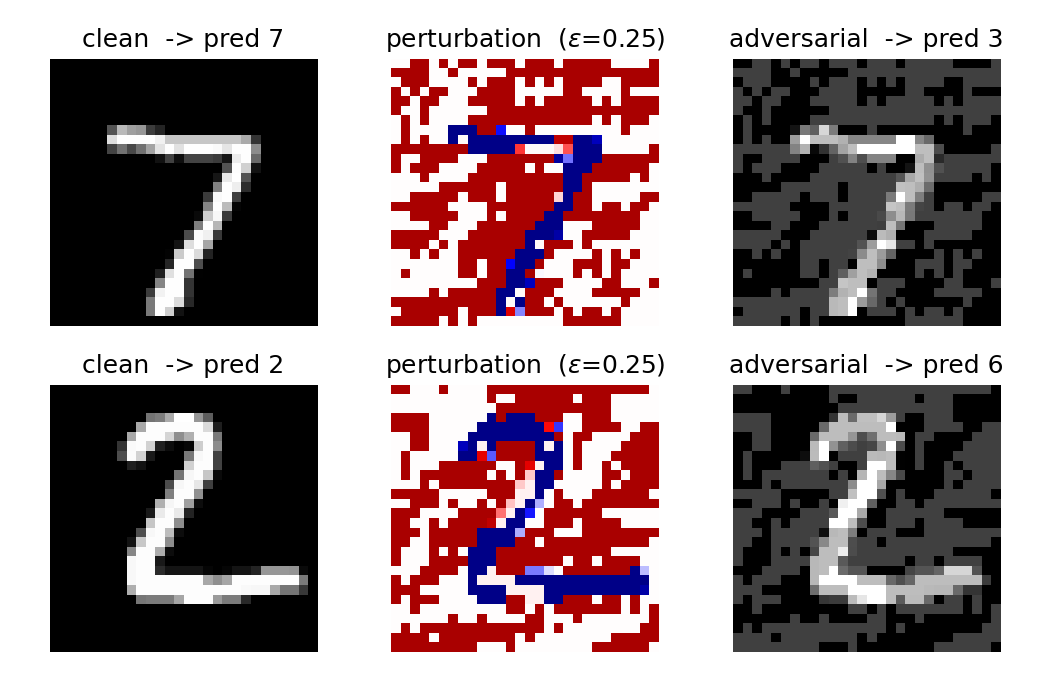
\includegraphics[width=\columnwidth]{outputs/fig1_samples.png}
  \caption{Original, perturbation, and FGSM adversarial examples ($\varepsilon\!=\!0.25$). The perturbation (center) amplified by a divergent color map; the resulting adversarial image (right) is visually close to the original yet flips the model's prediction.}
  \label{fig:samples}
\end{figure}

\textbf{Robustness sweep.} Table~\ref{tab:acc} reports accuracy across the budget grid; Figure~\ref{fig:curves}(a) plots the same data, and Figure~\ref{fig:curves}(b) breaks the standard-model accuracy at $\varepsilon\!=\!0.2$ down by digit class.

\begin{table}[h!]
  \centering\small
  \setlength{\tabcolsep}{3.5pt}
  \begin{tabular}{@{}cccc c@{}}
    \toprule
    $\varepsilon$ & FGSM / std & PGD / std & FGSM / rob & PGD / rob \\
    \midrule
    0.00 & 98.88 & 98.88 & 93.03 & 93.03 \\
    0.05 & 95.29 & 93.64 & 91.31 & 91.09 \\
    0.10 & 84.79 & 69.20 & 89.53 & 88.38 \\
    0.15 & 60.62 & 21.75 & 87.48 & 85.56 \\
    0.20 & 31.87 & \phantom{0}2.36 & 85.90 & 82.95 \\
    0.25 & 10.46 & \phantom{0}2.36 & 84.78 & 82.95 \\
    0.30 & \phantom{0}2.26 & \phantom{0}2.36 & 83.67 & 82.95 \\
    \bottomrule
  \end{tabular}
  \caption{Test accuracy (\%) of the standard and PGD adversarially trained CNN under FGSM and PGD-20 attacks across the $L_\infty$ budget grid.}
  \label{tab:acc}
\end{table}

\begin{figure}[h!]
  \centering
  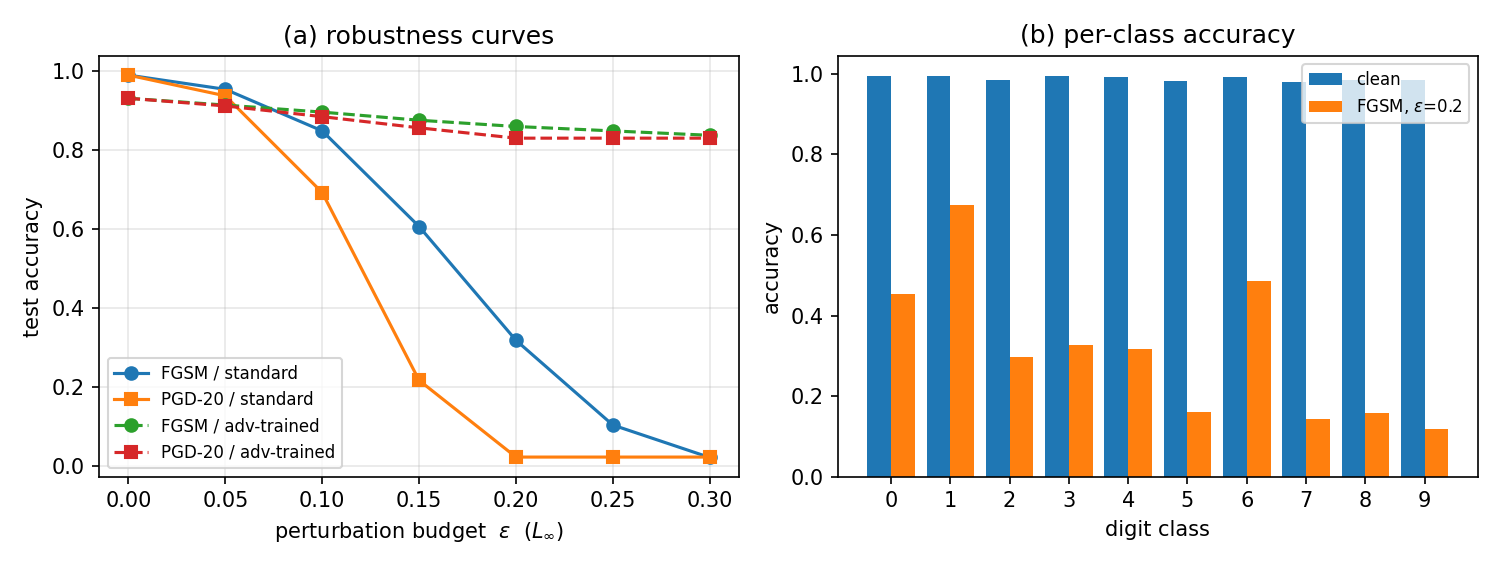
\includegraphics[width=\columnwidth]{outputs/fig2_curves.png}
  \caption{(a)~Robustness vs.\ perturbation budget $\varepsilon$ for the two models and two attacks. (b)~Per-class accuracy at $\varepsilon\!=\!0.2$ for the standard model, revealing pronounced heterogeneity across digits.}
  \label{fig:curves}
\end{figure}

\textbf{Error structure.} Figure~\ref{fig:confusion} contrasts the confusion matrix before and after FGSM attack at $\varepsilon\!=\!0.2$ on the standard model. The clean diagonal collapses, and errors concentrate into a few ``attractor'' columns (notably 1, 6, 9), often classes differing from the true class by a single stroke.

\begin{figure*}[t]
  \centering
  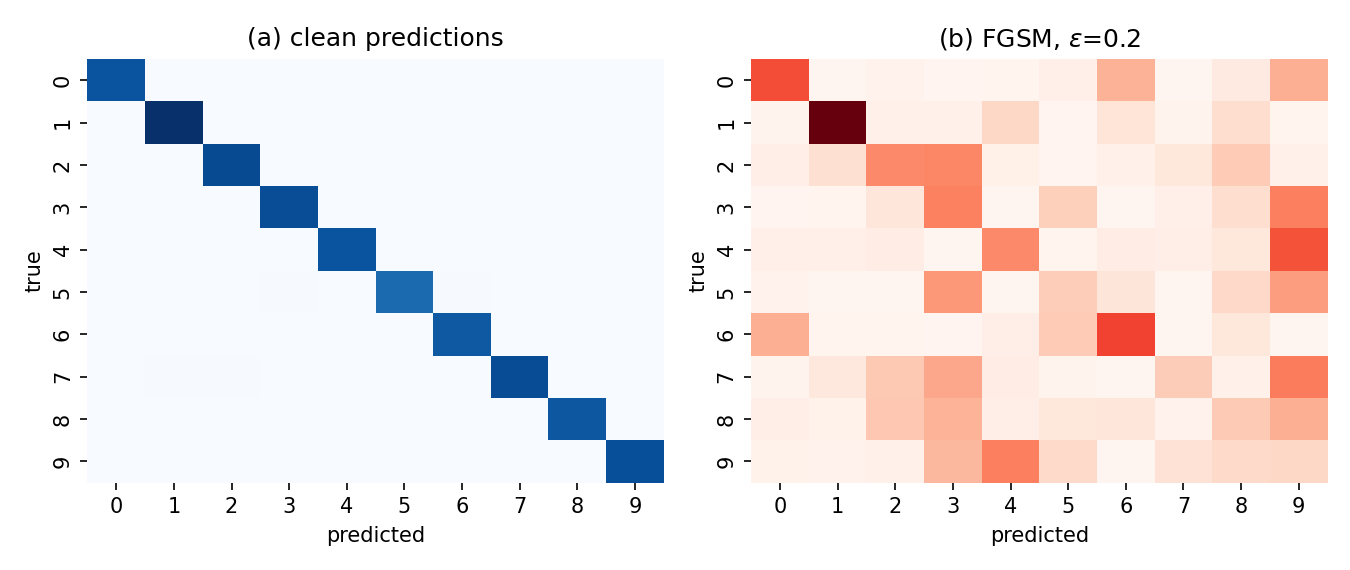
\includegraphics[width=0.70\textwidth]{outputs/fig3_confusion.png}
  \caption{Confusion matrices before (blue) and after (red) a white-box FGSM attack at $\varepsilon\!=\!0.2$ on the standard model. Under attack, errors concentrate into a few ``attractor'' classes rather than scattering uniformly, indicating structured rather than random failure.}
  \label{fig:confusion}
\end{figure*}

\textbf{Compute cost.} Table~\ref{tab:cost} contrasts the wall-clock cost of the three attacks on 1\,024 images on the RTX~2050. PGD-20---the standard evaluation adversary---is $24\times$ more expensive than FGSM, making attack strength a routine engineering trade-off during model assurance.

\begin{table}[h!]
  \centering\small
  \begin{tabular}{@{}lrrr@{}}
    \toprule
    Attack & Iterations & Time (s) / 1024 & Relative \\
    \midrule
    FGSM  & 1  & 0.034 & \phantom{0}1.00$\times$ \\
    PGD   & 7  & 0.235 & \phantom{0}6.90$\times$ \\
    PGD   & 20 & 0.817 & 24.03$\times$ \\
    \bottomrule
  \end{tabular}
  \caption{Wall-clock cost of each attack on 1\,024 MNIST test images (NVIDIA RTX 2050).}
  \label{tab:cost}
\end{table}

\textbf{Findings.} (i)~PGD dominates FGSM on the standard model at every $\varepsilon$; the gap grows from $1.65$ to $38.87$\,pp between $\varepsilon\!=\!0.05$ and $0.15$ and collapses thereafter as both attacks approach zero accuracy (Table~\ref{tab:acc}). (ii)~Adversarial training restores $\ge\!82.95\%$ accuracy under PGD-20 at $\varepsilon\!=\!0.3$, reproducing~\citet{madry2018towards} at small scale. (iii)~Robustness is \textbf{non-uniform across classes} (Figure~\ref{fig:curves}b): at $\varepsilon\!=\!0.2$, digit~1 retains $67.6\%$ accuracy while digit~9 falls to $11.8\%$. Digits with more visual ``competitors'' are attacked first, supporting the view that adversarial error concentrates along decision-boundary geometry rather than distributing uniformly. (iv)~PGD-20's $24\times$ compute cost over FGSM (Table~\ref{tab:cost}) matters when adversarial evaluation is a routine step in a CI pipeline. (v)~Adversarial training took $109.4$\,s vs.\ $12.8$\,s for clean training, an $8.5\times$ total overhead ($5\times$ per epoch from the PGD-7 inner loop plus $1.67\times$ from the longer schedule).

\section{Ethical Considerations}
\label{sec:ethics}

Adversarial ML is \textbf{dual-use}. Offensively, the same techniques that fool a stop-sign classifier can (i)~enable impersonation against biometric checkpoints, (ii)~craft deepfakes that evade forensic classifiers, or (iii)~bypass spam and malware filters. Publishing attack code therefore risks arming malicious actors. Yet \emph{withholding} attacks leaves defenders blind: \citet{nist2021aml} explicitly recommend disclosure because ``security through obscurity'' systematically favors attackers. A responsible stance---adopted here---reproduces published attacks on toy datasets while foregrounding defense. A second ethical axis concerns \textbf{fairness}: a robust classifier that has inherited demographic skew~\citep{bagdasaryan2019differential} can be attacked \emph{differentially} across groups, compounding fairness harms. Our per-class analysis (Figure~\ref{fig:curves}b) is the MNIST analogue of this concern---robustness gaps spanning $55.8$\,pp between easy and hard classes---motivating the reporting of \emph{worst-class} robustness alongside average accuracy.

\section{Future Directions}
\label{sec:future}

Three frontiers appear most promising. \textbf{(1)~Certified defenses.}~\citet{cohen2019certified} convert a base classifier into a provably robust one by majority-voting over Gaussian-noised inputs; the certificate scales favorably to ImageNet. \textbf{(2)~Physically realizable attacks.} Beyond digital perturbations, the \emph{Expectation-over-Transformation} framework produces adversaries robust to real-world imaging pipelines~\citep{athalye2018obfuscated}, motivating sensor-level and deployment-time defenses. \textbf{(3)~Foundation-model robustness.} Large pretrained models exhibit emergent behaviors under adversarial prompting~\citep{zou2023universal}; extending the $L_\infty$ threat model to text, speech, and multi-modal inputs is an open and socially consequential direction.

\section{Conclusion}
\label{sec:conclusion}

We surveyed the landscape of adversarial machine learning and empirically reproduced FGSM, PGD, and Madry-style adversarial training on MNIST under a modest compute budget. The quantitative picture (Tables~\ref{tab:acc}--\ref{tab:cost}, Figures~\ref{fig:samples}--\ref{fig:confusion}) confirms that (i)~adversarial vulnerability is severe for standardly trained networks, (ii)~adversarial training is an effective, if computationally costly, remediation, (iii)~the benefit is non-uniform across classes, and (iv)~strong attacks are $24\times$ more expensive than weak ones. Trustworthy AI will require combining such empirical defenses with certified guarantees, physical-world evaluation, and careful dual-use ethics.

{\scriptsize
\setlength{\bibsep}{1.5pt}
\bibliographystyle{unsrtnat}
\begin{thebibliography}{13}

\bibitem[Athalye et~al.(2018)]{athalye2018obfuscated}
A.~Athalye, N.~Carlini, and D.~Wagner.
\newblock Obfuscated gradients give a false sense of security.
\newblock In \emph{ICML}, 2018.

\bibitem[Bagdasaryan et~al.(2019)]{bagdasaryan2019differential}
E.~Bagdasaryan, O.~Poursaeed, and V.~Shmatikov.
\newblock Differential privacy has disparate impact on model accuracy.
\newblock In \emph{NeurIPS}, 2019.

\bibitem[Cohen et~al.(2019)]{cohen2019certified}
J.~Cohen, E.~Rosenfeld, and Z.~Kolter.
\newblock Certified adversarial robustness via randomized smoothing.
\newblock In \emph{ICML}, 2019.

\bibitem[Eykholt et~al.(2018)]{eykholt2018robust}
K.~Eykholt et~al.
\newblock Robust physical-world attacks on deep learning visual classification.
\newblock In \emph{CVPR}, 2018.

\bibitem[Goodfellow et~al.(2015)]{goodfellow2015explaining}
I.~J. Goodfellow, J.~Shlens, and C.~Szegedy.
\newblock Explaining and harnessing adversarial examples.
\newblock In \emph{ICLR}, 2015.

\bibitem[Grosse et~al.(2017)]{grosse2017adversarial}
K.~Grosse et~al.
\newblock Adversarial examples for malware detection.
\newblock In \emph{ESORICS}, 2017.

\bibitem[Madry et~al.(2018)]{madry2018towards}
A.~Madry, A.~Makelov, L.~Schmidt, D.~Tsipras, and A.~Vladu.
\newblock Towards deep learning models resistant to adversarial attacks.
\newblock In \emph{ICLR}, 2018.

\bibitem[NIST(2021)]{nist2021aml}
NIST.
\newblock \emph{Adversarial Machine Learning: A Taxonomy and Terminology of Attacks and Mitigations}, NISTIR 8269 draft, 2021.

\bibitem[Papernot et~al.(2016)]{papernot2016practical}
N.~Papernot, P.~McDaniel, I.~Goodfellow, et~al.
\newblock Practical black-box attacks against machine learning.
\newblock In \emph{AsiaCCS}, 2016.

\bibitem[Sharif et~al.(2016)]{sharif2016accessorize}
M.~Sharif, S.~Bhagavatula, L.~Bauer, and M.~Reiter.
\newblock Accessorize to a crime: Real and stealthy attacks on state-of-the-art face recognition.
\newblock In \emph{CCS}, 2016.

\bibitem[Szegedy et~al.(2014)]{szegedy2014intriguing}
C.~Szegedy et~al.
\newblock Intriguing properties of neural networks.
\newblock In \emph{ICLR}, 2014.

\bibitem[Xu et~al.(2018)]{xu2018feature}
W.~Xu, D.~Evans, and Y.~Qi.
\newblock Feature squeezing: Detecting adversarial examples in deep neural networks.
\newblock In \emph{NDSS}, 2018.

\bibitem[Zou et~al.(2023)]{zou2023universal}
A.~Zou et~al.
\newblock Universal and transferable adversarial attacks on aligned language models.
\newblock \emph{arXiv:2307.15043}, 2023.

\end{thebibliography}
}

\end{document}
